%
% spline.tex -- spline.tex
%
% (c) 2021 Prof Dr Andreas Müller, OST Ostschweizer Fachhochschule
%
\bgroup
\definecolor{darkgreen}{rgb}{0,0.6,0}
\begin{frame}[t]
\setlength{\abovedisplayskip}{5pt}
\setlength{\belowdisplayskip}{5pt}
\frametitle{Spline-Interpolation}
\vspace{-20pt}
\begin{columns}[t,onlytextwidth]
\begin{column}{0.60\textwidth}
\vspace{-10pt}
\begin{center}
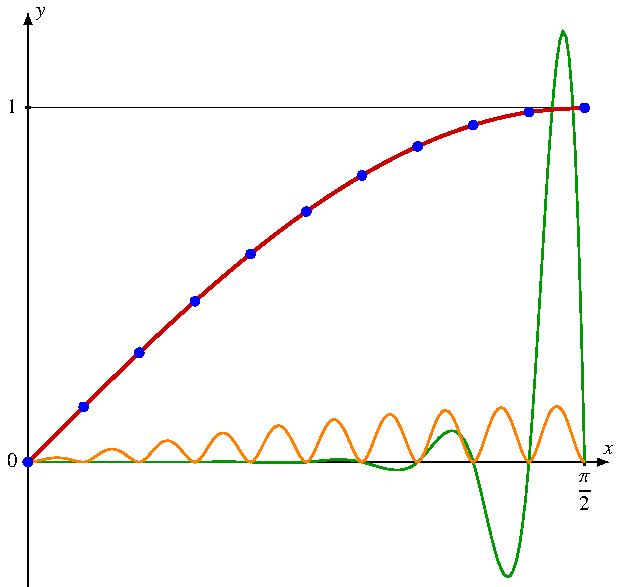
\includegraphics[width=\textwidth]{../../buch/chapters/030-nichtdiff/images/sinspline.pdf}
\end{center}
\end{column}
\begin{column}{0.36\textwidth}
\begin{block}{Parameter}
\begin{itemize}
\item
$f(x) = \sin x$
\item
11 Stützstellen $x_k = \frac{k}{10}\pi$
\item
$y(x_k) = \sin x_k$, $k=0,\dots,10$
\end{itemize}
\vspace*{-10pt}
\end{block}
\begin{block}{Spline-Interpolation}
$y(x_k) = \sin x_k$, $k=0,\dots,10$

Steigungen $s_k$ aus % der Bedingung
$\int_a^b y''(x)^2\,dx\to\text{Minimum}$
\\[5pt]
(Fehler {\color{darkgreen}grün}, $1000 \times$)
\end{block}
\vspace*{-2pt}
\uncover<2->{%
\begin{block}{Hermite-Interpolation}
Steigungen $s_k = \cos x_k$
\\[5pt]
(Fehler {\color{orange}orange}, $1000\times$)
\end{block}}
\end{column}
\end{columns}
\end{frame}
\egroup
